\documentclass{article}
\usepackage{booktabs}
\usepackage{graphicx}
\usepackage{amsmath}
\title{基于 t-SNE 特征的船舶目标分类研究}
\author{测试用稿}
\begin{document}
\maketitle

\section{实验结果}
我们在三个数据集上对比了多种方法。如表~\ref{tab:main} 所示，本文方法在准确率与 F1 上均优于基线。

\begin{table}[h]
\centering
\caption{各方法的分类性能对比（\%）与推理耗时（s）}
\label{tab:main}
\begin{tabular}{lccc}
\toprule
方法 & 准确率 & F1 & 耗时 \\
\midrule
SVM   & 85.5 & 80.5 & 12.5 \\
RF    & 86.5 & 81.5 & 13.5 \\
KNN   & 87.5 & 82.5 & 14.5 \\
CNN   & 88.5 & 83.5 & 15.5 \\
LSTM  & 89.5 & 84.5 & 16.5 \\
Ours  & 90.5 & 85.5 & 17.5 \\
\bottomrule
\end{tabular}
\end{table}

在用户主观评测中，平均评分为 2.37（n = 10，5 分制）。
另有一组审稿评分为 2.0 $\pm$ 3.0（n = 20，1--7 分制）。

图~\ref{fig:tsne} 给出了特征的 t-SNE 可视化，可见各类别聚类清晰、边界分明。

\begin{figure}[h]
\centering
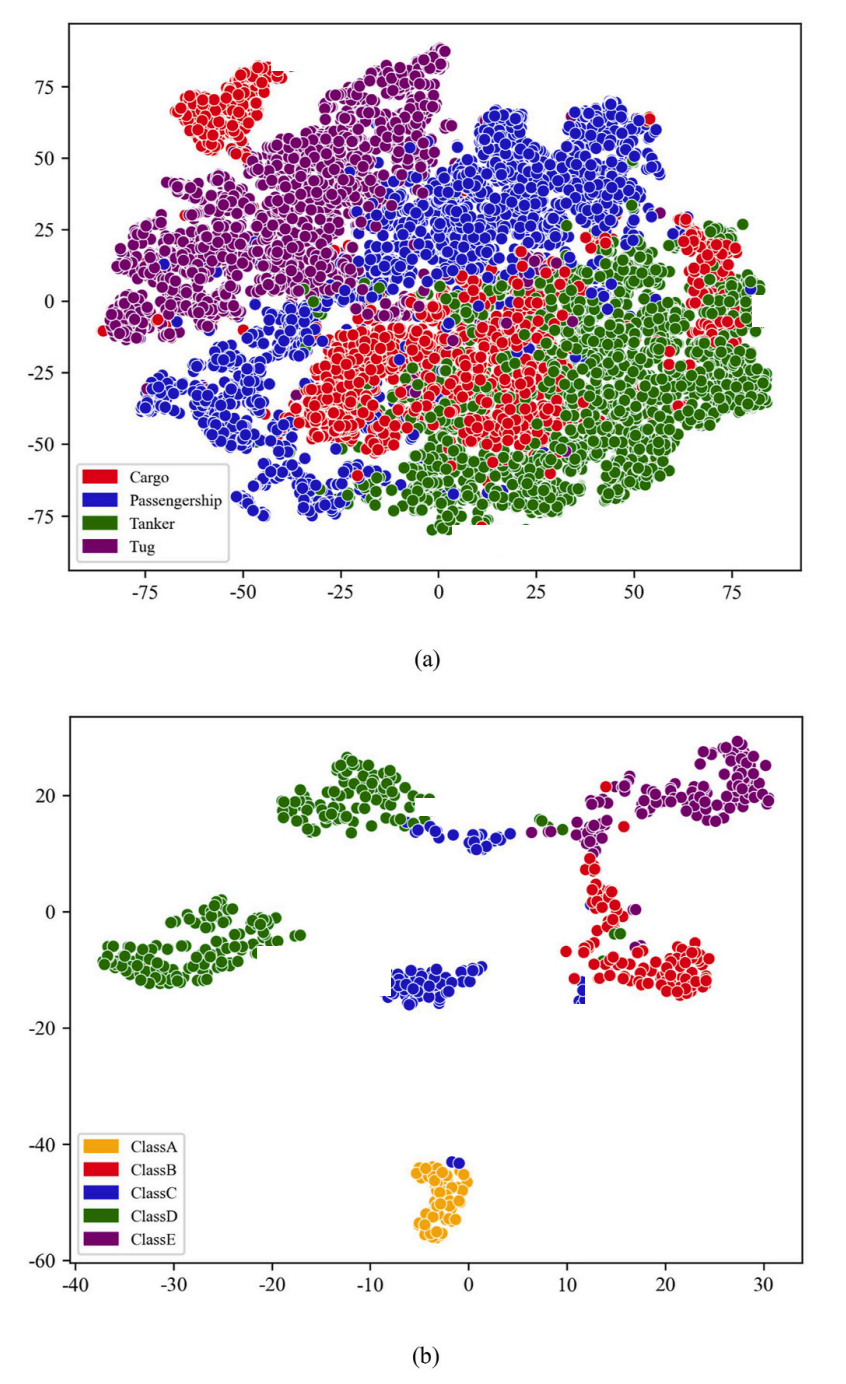
\includegraphics[width=0.5\textwidth]{test.png}
\caption{特征的 t-SNE 可视化：(a) 四类船舶；(b) 五类细分。}
\label{fig:tsne}
\end{figure}

\section{消融实验}
表~\ref{tab:ablation} 为消融结果。

\begin{table}[h]
\centering
\caption{消融实验（\%）}
\label{tab:ablation}
\begin{tabular}{lcc}
\toprule
配置 & 准确率 & F1 \\
\midrule
w/o A & 88.2 & 83.1 \\
w/o B & 88.2 & 83.1 \\
完整模型 & 90.5 & 85.5 \\
\bottomrule
\end{tabular}
\end{table}

\end{document}
